\section{Разработка параллельного алгоритма реконструкции поверхности}
\subsection{Предложенный параллельный метод}
Параллельный вариант, модифицированного алгоритма MLS с использованием MPI, описан в алгоритме 1. Алгоритм предполагает что облако точек равномерно распределено по всем процессам \ref{fig:decomposition}. Поэтому часть P, доступная локально в процессе u, обозначается через $P^{(u)}$. Через $P_l^{u}$, $P_r^{u}$ обозначены левая и правая граница частей облака точек. Они последовательно получаются от соседних процессов обменами по топологии кольцо. Дополнительных коммуникаций не требуется, а остальные вычисления выполняются локально. В цикле по локальному облаку точек $P^{(u)}$ выполняется процедура проецирования MLS: сначала создается локальная эталонная плоскость H для точки $p_j$. Проекция $p_j$ на H определяет начало координат q. Затем вычисляется локальная полиномиальная аппроксимация g высот $f_j$ точек $p_j$ над H. Проекция $p_j$ на g является результатом работы алгоритма MLS. \\*
\textbf{Алгоритм 1}  Параллельный метод движущихся наименьших квадратов с MPI и OpenMP \\*
\textbf{Вход:} набор точек $P = \{p_i\}$ $i = 1..n$ \\*
\textbf{Выход:} поверхность представленная набором точек \\*
1: \textbf{for each} process u \textbf{do} \\*
2: \quad $P^{(u)} = read(P)$ // каждый процесс считывает свой сегмент облака точек $P^{(u)} = \{p_j\}$ $j = 1..m$ \\*
3: \quad $P\_l^{(u)} = send\_recv(P\_r^{(u-1)})$ // получение левой границы\\* 
4: \quad $P\_r^{(u)} = send\_recv(P\_l^{(u+1)})$ // получение правой границы\\*
5: \quad\textbf{pragma omp parallel for} \\*
6: \quad\textbf{for each} point $j = 1..m $ \textbf{do}\\*
7: \quad\quad$H = generate\_plane(p_j)$ \\*
8: \quad\quad$g = generate\_local\_polynomial\_approximation(H)$ \\*
9: \quad\quad$result\_point = project\_on\_polynom(p_j, polynom)$ \\*
10: \quad\textbf{end for} \\*

При исследовании информационной структуры алгоритма был построен граф информационной зависимости \ref{fig:information}. Из графа видно отсутствие информационной зависимости между точками запроса, поэтому итерации по циклу из локального набора точек $P^{(u)}$ были распараллелены средствами OpenMP (строчка 5 алгоритма 1). 

\begin{figure}[h]
    \centering
    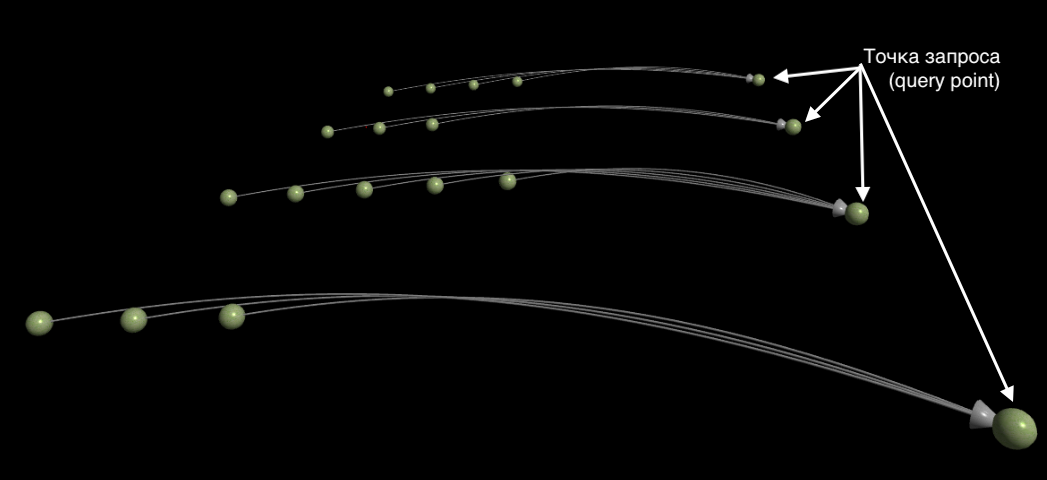
\includegraphics[width=0.7\textwidth, height=5cm]{images/graph.png}
    \caption{Граф информационной зависимости MLS.}
    \label{fig:information}
\end{figure}

\begin{figure}[h]
    \centering
    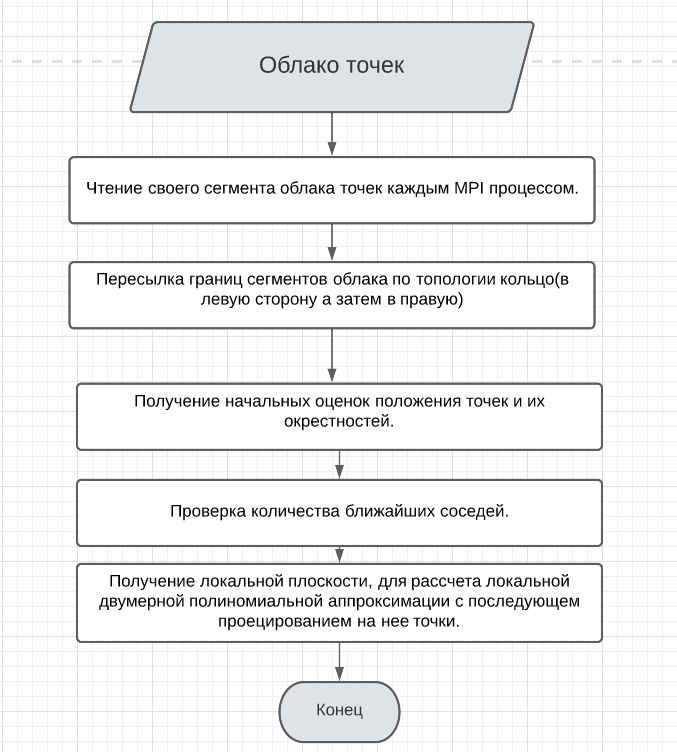
\includegraphics[scale=0.9]{1.png}
    \caption{Блок-схема параллельной реализации алгоритма}
    \label{fig:mesh1}
\end{figure}


\begin{figure}[h]
  \centering
  \subbottom[$np = 1$]{%
    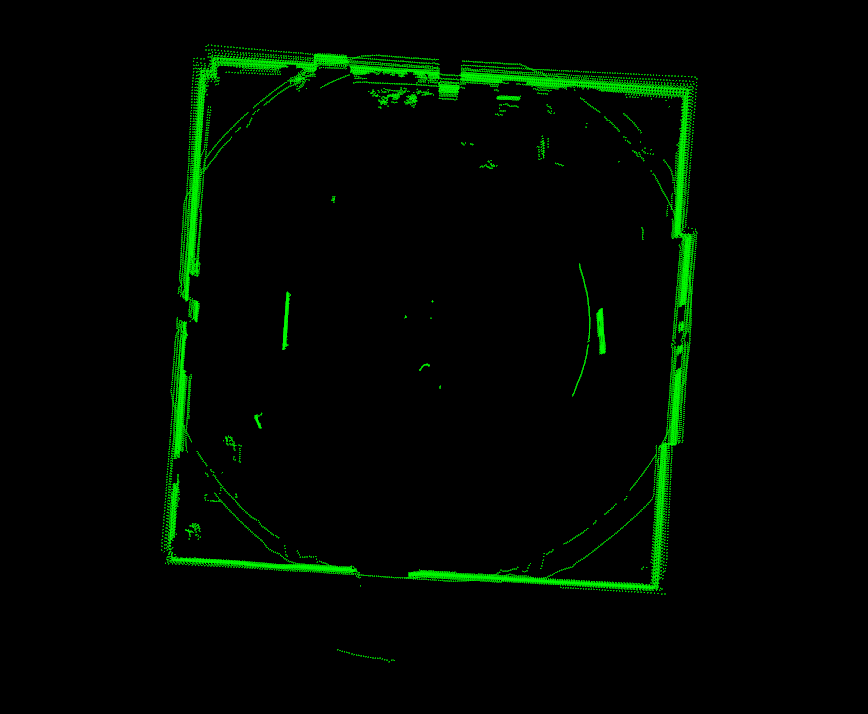
\includegraphics[width=0.4\textwidth, height=7cm]{images/3.png}}
  \subbottom[$np = 4$]{%
    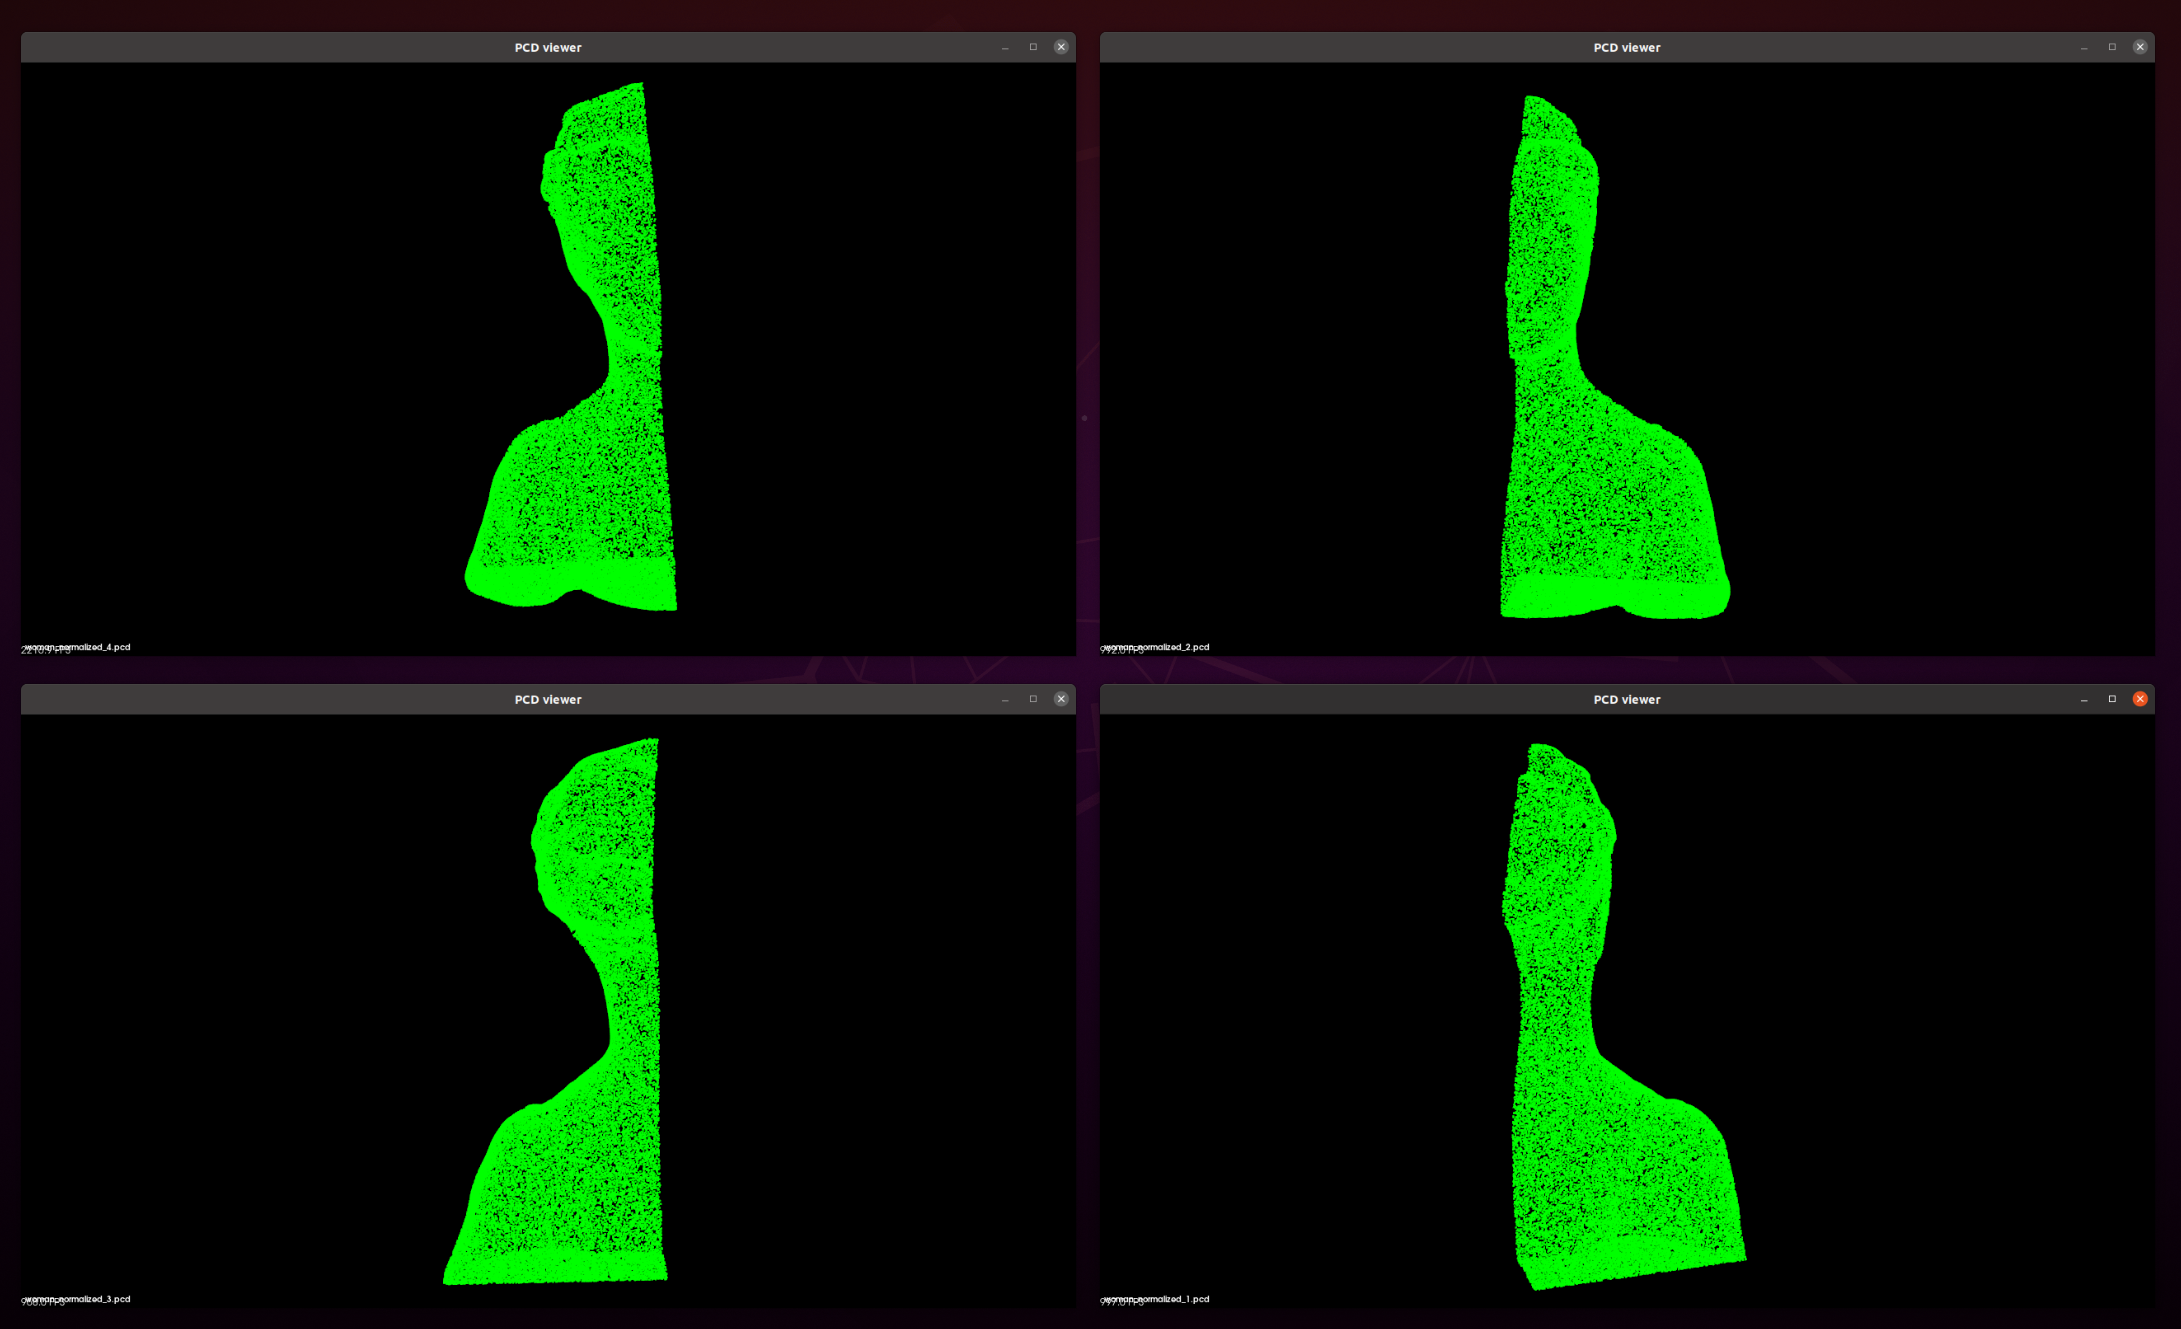
\includegraphics[width=0.58\textwidth, height=7cm]{images/2.png}}
  \caption{Распределение сегментов облака точек по процессам}
  \label{fig:decomposition}
\end{figure}

\clearpage



\subsection{Вычислительная сложность}
Для эффективного поиска точек попадающих в R окрестность используется структура данных k-d дерево. Вычислительная сложность построения k-d-дерева порядка: $O(n*k*log(n))$. Здесь k = 3 и имеет значение размерности. Несбалансированное k-d-дерево можно построить за $O(n(k+log(n)))$. У нас есть n точек, каждая вставляется за логарифмическую сложность. Слагаемое $O(nk)$ имеет следующее значение: Перед построением дерева находится минимум и максимум по каждой размерности для последующего равномерного разбиения. В случае сбалансированного дерева применяется предварительная сортировка по всем размерностям сложностью порядка $O(nlog n)$.
Поиск точек в окрестности R имеет сложность порядка $O(log n)$.
Метод наименьших квадратов для поиска плоскости имеет сложность порядка $O(C^2*m)$ $ (C = 4)$. Здесь С имеет значение количества параметров, и равно 4‑м поскольку мы ищем плоскость.
Интерполяция полиномом имеет сложность порядка $O(m^2)$, где m имеет значение количества точек попавших в R окрестность.

\begin{table}[h]
\centering
\begin{tabular}{||p{7cm}||p{9.3cm}||}
\hline
Этап алгоритма & сложность\\
\hline\hline
Построение k-d-дерева &  $O(n \cdot k \cdot log(n))$ (Несбалансированное $O(n(k+log(n)))$ ) \\
\hline
Поиск точек в окрестности R & $O(log n)$  \\
\hline
Метод наименьших квадратов & $O(C^2 \cdot m) (C = 4)$\\
\hline
Интерполяция полиномом & $O(m^2)$ \\
\hline
Проекция точки на полином & $O(1)$ \\
\hline
\end{tabular}
\caption{Вычислительная сложность основных этапов алгоритма}
\label{table:complexity}
\end{table}

Итоговая амортизационная вычислительная сложность алгоритма: 

$O(n \cdot k \cdot log(n))$  + n $\cdot$ ($O(log n)$ + $O(C^2 \cdot m)$ + $O(m^2)$ + $O(1)$)